\documentclass{article}
\usepackage{latexsym}
\usepackage[utf8]{inputenx}
\usepackage[spanish]{babel}
\usepackage{graphicx}
\usepackage{anysize}
\usepackage{amsmath}
\usepackage{amssymb}
\usepackage{float}
\setlength{\skip\footins}{5cm}
\usepackage{lscape}
\usepackage{verbatim}
\usepackage{moreverb}
\usepackage{url}
\usepackage{enumitem}
\usepackage{multicol}
\let\verbatiminput=\verbatimtabinput
\usepackage[nottoc,numbib]{tocbibind}
\setcounter{tocdepth}{4}
\setcounter{secnumdepth}{4}
\usepackage{listings}

\marginsize{2cm}{2cm}{.5cm}{3cm} 

\begin{document}

\begin{titlepage}

\newcommand{\HRule}{\rule{\linewidth}{0.5mm}} % Defines a new command for the horizontal lines, change thickness here

\center % Center everything on the page
 
%----------------------------------------------------------------------------------------
%	HEADING SECTIONS
%----------------------------------------------------------------------------------------

\textsc{\LARGE Universidad De Buenos Aires}\\[1.5cm] % Name of your university/college
\textsc{\Large Facultad De Ingeniería}\\[0.5cm] % Major heading such as course name
\textsc{\large 66.20 Organización De Computadoras}\\[0.5cm] % Minor heading such as course title

%----------------------------------------------------------------------------------------
%	TITLE SECTION
%----------------------------------------------------------------------------------------

\HRule \\[0.4cm]
{ \huge \bfseries Trabajo Práctico 0}\\[0.4cm] % Title of your document
\HRule \\[1.5cm]
 
%----------------------------------------------------------------------------------------
%	AUTHOR SECTION
%----------------------------------------------------------------------------------------

% If you don't want a supervisor, uncomment the two lines below and remove the section above
\Large \emph{Integrantes:}\\
Gonzalo \textsc{Beviglia} - 93144\\ % Your name
Federico \textsc{Quevedo} - 93159\\ % Your name
Damián \textsc{Manoff} - 93169\\[5cm] % Your name

%----------------------------------------------------------------------------------------
%	LOGO SECTION
%----------------------------------------------------------------------------------------


\includegraphics[scale=0.5]{UBA.jpg}\\[1cm] % Include a department/university logo - this will require the graphicx package

%----------------------------------------------------------------------------------------
%	DATE SECTION
%----------------------------------------------------------------------------------------

{\large \text \em {10 de Septiembre de 2013}}\\[3cm] % Date, change the \today to a set date if you want to be precise
 
%----------------------------------------------------------------------------------------

\vfill % Fill the rest of the page with whitespace

\end{titlepage}

	\tableofcontents
		
\newpage

\section{Diseño e implementación}

Uno de los principales limitantes de las soluciones que pudimos implementar era el largo del archivo a invertir, ya que este podia llegar a ocupar mucho lugar en la memoria. Buscamos mejorar esta situación leyendo e invirtiendo de a un archivo por vez, para evitar tener mas de uno en memoria. También evitamos tener que declarar otro espacio de memoria del mismo tamaño del archivo original, donde iria la cadena invertida, haciendo una inversion in situ de la cadena, es decir, sobre la misma memoria reservada a donde se cargo el archivo. Esto ademas de ahorrarnos duplicar la memoria usada nos ahorra el tiempo de reservar la misma. Sobre la cadena original se realizan swaps espejados hasta llegar a la cadena invertida.

\section{Performance}

La performance se evaluó invirtiendo el libro ``El Príncipe'' de Nicolás Maquiavelo, y se comparó
la performance del comando realizado para este trabajo práctico con la del comando unix \emph{rev}.
El tamaño de dicho texto en formato de texto plano es de 305864 bytes (298KB).

Los tiempos se midieron utilizando el comando Unix \emph{time}.

\subsection{Tiempo \emph{ownRev}}

\begin{verbatim}
real	0m0.539s

user	0m0.008s

sys	0m0.016s
\end{verbatim}



\subsection{Tiempo Unix \emph{rev}}

\begin{verbatim}
real	0m0.540s

user	0m0.012s

sys	0m0.024s
\end{verbatim}

\subsection{Comparación grafica}

Los textos utilizados para esta comparación fueron: 
\begin{itemize}
\item The Divine Comedy - Dante Alighieri (627KB)
\item Adventures of Huckleberry Finn - Mark Twain (596KB)
\item Les Miserables - Victor Hugo (3.2MB)
\item Metamorphosis - Franz Kafka (139KB)
\item The Prince - Nicolo Machiavelli (299KB)
\end{itemize}

\begin{figure}[h!]
  \caption{Comparacion entre rev de Unix y nuestro ``ownRev''}
  \centering
    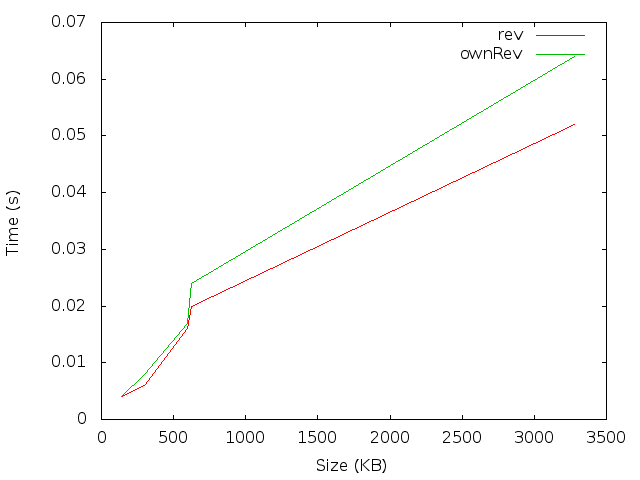
\includegraphics[width=0.5\textwidth]{TestFiles/times.png}
\end{figure}

\newpage

\section{Compilación del programa}

Para el compilado del programa hicimos el siguiente makefile:

\lstinputlisting{Makefile}

La ejecución normal de este make file produce el archivo ejecutable y ademas elimina los intermediarios.

Se puede tambien llamar pasando como parametro el nombre del archivo intermediario para generarlo, o el nombre del ejecutable, que realizara lo mismo que la ejecución por defecto pero sin eliminar el intermediario.

Para corroborar que no se estuviera perdiendo memoria tambien incluimos el parametro \(memCheck\) que corre el programa con valgrind informando si hubo o no alguna perdida.

Desde el mismo makefile tambien incluimos la posibilidad de correr las pruebas, y por ultimo, la de eliminar los archivos generados, tanto intermediarios como programa final.

\section{Pruebas}

Para las pruebas hicimos el siguiente script de bash:

\lstinputlisting[language=Bash]{TestFiles/tests.sh}

Se toman lineas de un archivo, en este caso llamado test, y se las invierte usando tanto nuestro programa como el comando \( rev \) de linux, si los resultados son iguales la prueba es valida.

\section{C\'odigo Fuente}

\subsection{C\'odigo fuente C}

\lstinputlisting[language=C]{ownRev.c}

\subsection{C\'odigo assembly MIPS}

A continuaci\'on se detallará el c\'odigo assembly para la arquitectura MIPS de nuestro programa en C

\lstinputlisting{tp0v2.s}

\section{Conclusiones}

Luego de realizar este trabajo práctico, podemos concluir que el comando ``rev'' es sencillo de implementar al nivel al que estuvimos interesados a la hora de desarrollarlo. Sería interesante indagar el c\'odigo fuente del comando original de Linux para ver que tan alejados estamos de una implementación óptima.

Se nos ocurre que, por ejemplo, el comando ``rev'' debe hacer un checkeo de errores más exhaustivo, que a nosotros, como alumnos, quizas no fuimos capaces de observarlos como posibles.

Es interesante ver como los tiempos de ejecución para ambas implementaciones son similares, siendo estos tiempos obtenidos mediante la reversión de archivos de texto grandes, sin imprimir el resultado por pantalla.

En nuestra opinion, uno de los elementos más importantes y más útiles a la hora del desarrollo y la corrección del trabajo práctico, fue el uso de las pruebas automatizadas. Fueron la herramienta que nos permitió consolidar una base de código en funcionamiento para luego poder optimizar al programa y corregir errores indicados por el corrector.

Con lo que lleva a la asignatura se nota claramente una diferencia entre en c\'odigo assembly de MIPs y el c\'odigo del programa en C. Cuando en C tenemos casi 200 lineas de c\'odigo en assembly llegamos casi a las 600 es decir el triple de lineas de c\'odigo por el mismo programa. Claramente notamos lo dificultoso y tedioso que es programar en este lenguaje, pero el poder que tiene es muchisimo mayor, ya que notamos paso a paso , linea a linea como funciona correctamente nuestro trabajo, y en caso de haber \textit{Bugs} que a simple vista en C no podriamos encontrar, aca claramente hallar\'iamos el problema. Es decir, cuando no nos quede otra alternativa para solucionar los problemas, seguramente sabiendo leer el c\'odigo de m\'aquina tendremos un panorama mas claro del problema y as\'i talvez llegar a una soluci\'on factible.

\end{document}
